\section{Fourierreihen periodischer Funktionen}
	\subsection{Bausteine}
		\textbf{Idee:}\\[3pt]
		$T$-Periodische, mit Limes stückweise stetigen Funktionen, durch Aufsummieren ebenfalls periodischer Basisfunktionen
		(sin, cos) zu approximieren.\\[3pt]

		\textbf{Basisfunktionen:}\\[3pt]
		\begin{minipage}[t]{0.5\textwidth}
			\begin{tabular}{llll}
				Konstante: & $cos(0 \cdot \omega_{f} t) = 1$ & &\\[3pt]
				$1 \times$ Frequenz $f$  & $\cos(1 \cdot \omega_{f} t)$ & ; & $\sin(1 \cdot \omega_{f} t)$\\[3pt]
				$2 \times$ Frequenz $f$: & $\cos(2 \cdot \omega_{f} t)$ & ; & $\sin(2 \cdot \omega_{f} t)$\\[3pt]
				$3 \times$ Frequenz $f$: & $\cos(3 \cdot \omega_{f} t)$ & ; & $\sin(3 \cdot \omega_{f} t)$\\[3pt]
				usw. & & &\\[3pt]
			\end{tabular}
		\end{minipage}
		\begin{minipage}[t]{0.2\textwidth}
			
		\end{minipage}
		\begin{minipage}[t]{0.3\textwidth}
			\fbox{
				\begin{tabular}{ll}
					Frequenz: & $f = \dfrac{1}{T}$\\[7pt]
					Kreisfrequenz: & $\omega_f = 2 \pi f$\\[3pt]
					Periodendauer: & $T = \dfrac{2 \pi}{\omega_f} = \dfrac{1}{f}$\\[6pt]
					Nullphasenwinkel: & $\varphi$\\[6pt]
				\end{tabular}
			}
		\end{minipage}
	
	\subsection{Berechnung der Fourierkoeffizienten (in $\mathbb{R}$)}
		\textbf{Die Funktion $f(t)$ soll durch folgende Linearkombination dargestellt werden:}\\[3pt]
		\fbox{$FR[f(t)] = \dfrac{a_0}{2} + \sum\limits_{n=1}^{\infty} [a_n \cdot \cos(n \omega_f t) + b_n \sin(n \omega_f t)]$}\\[3pt]
		\begin{minipage}[t]{0.5\textwidth}
			\textbf{Berechnung von $a_0$, $a_n$ und $b_n$\\[1pt] (Fourierkoeffizienten):}\\[3pt]
			\begin{tabular}{|lll|l|}
				\hline
				$\displaystyle a_0$ & $=$ & $\displaystyle \dfrac{2}{T} \cdot \int\limits_{0}^{T} f(t) dt$ & $\displaystyle n = 0$\\[0.2pt]
				\hline
				$\displaystyle b_0$ & $\displaystyle =$ & $\displaystyle 0$ & $\displaystyle n = 0$\\
				\hline
				$\displaystyle a_n$ & $\displaystyle =$ & $\displaystyle \dfrac{2}{T} \cdot \int\limits_{0}^{T} f(t) \cdot \cos(n \omega_f t) dt$ & $\displaystyle n = 0, 1, 2, \cdots$\\
				\hline
				$\displaystyle b_n$ & $\displaystyle =$ & $\displaystyle \dfrac{2}{T} \cdot \int\limits_{0}^{T} f(t) \cdot \cos(n \omega_f t) dt$ & $\displaystyle n = 1, 2, 3, \cdots$\\
				\hline
			\end{tabular}
		\end{minipage}
		\begin{minipage}[t]{0.5\textwidth}
			\textbf{Orthogonalitätsbeziehungen:\\[1pt]}\\[3pt]
			\begin{tabular}{|l|}
				\hline
				$\displaystyle \int\limits_{0}^{T} \cos(m \omega_f t) \cdot \cos(n \omega_f t) dt = \left\lbrace 
					\begin{array}{ll}
						T & \text{für: } m = n = 0\\
						\dfrac{T}{2} & \text{für: } m = n > 0\\
						0 & \text{für: } m \neq n\\
					\end{array} \right.$\\[3pt]
				$\displaystyle \int\limits_{0}^{T} \sin(m \omega_f t) \cdot \sin(n \omega_f t) dt = \left\lbrace 
					\begin{array}{ll}
						\dfrac{T}{2} & \text{für: } m = n > 0\\
						0 & \text{für: } m \neq n\\
					\end{array} \right.$\\[3pt]
				$\displaystyle \int\limits_{0}^{T} \sin(m \omega_f t) \cdot \sin(n \omega_f t) dt = 0$\\[3pt]
				\hline
			\end{tabular}
		\end{minipage}
	
	\subsection{Sätze zur Berechnung der Fourierkoeffizienten}
		\subsubsection{Symmetrie}
			\begin{minipage}[t]{0.5\textwidth}
				\begin{tabular}{|c|c|}
					\hline
					\textbf{Gerade Funktion} & \textbf{Ungerade Funktion}\\[3pt]
					\hline
					\scalebox{0.45}{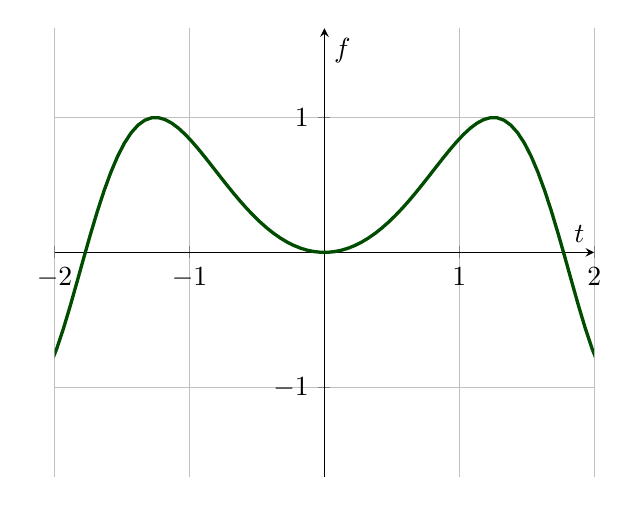
\begin{tikzpicture}
	\begin{axis}[axis lines=middle, axis equal, grid=both, xmin = -2, xmax = 2, ymin = -1, ymax = 1, xlabel = $t$, ylabel = $\operatorname{f}$]
		\addplot[black!70!green, very thick, samples = 200] {sin(deg(x^2))} node[above, red] at (10, 10) {$f$};
	\end{axis}
\end{tikzpicture}} & \scalebox{0.45}{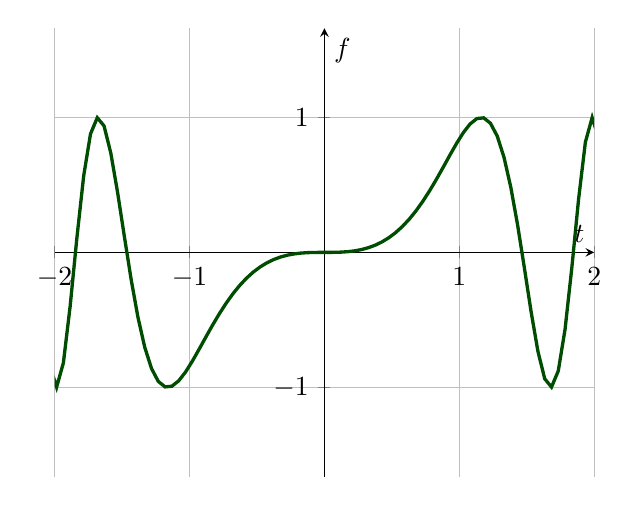
\begin{tikzpicture}
	\begin{axis}[axis lines=middle, axis equal, grid=both, xmin = -2, xmax = 2, ymin = -1, ymax = 1, xlabel = $t$, ylabel = $\operatorname{f}$]
		\addplot[black!70!green, very thick, samples = 200] {sin(deg(x^3))} node[above, red] at (100, 100) {$f$};
	\end{axis}
\end{tikzpicture}}\\[3pt]
					\hline
					achsensymmetrisch & punktsymmetrisch\\[3pt]
					$\displaystyle f(t) = f(-t)$ & $f(t) = -f(-t)$\\[3pt]
					\hline
					Beispiel: $\displaystyle \cos$ & Beispiel: $\sin$\\[3pt]
					\hline
					$\displaystyle \int\limits_{0}^{T} f(t) dt = 2 \int\limits_{0}^{T/2} f(t) dt$ & $\displaystyle \int\limits_{0}^{T} f(t) dt = 0$\\[3pt]
					\hline
				\end{tabular}
			\end{minipage}
			\begin{minipage}[t]{0.5\textwidth}
				\textbf{Rechnen mit geraden und ungeraden Funktionen:}\\[3pt]
				\begin{tabular}{|lclcl|}
					\hline
					gerade & $\cdot$ & gerade & $=$ & gerade\\[3pt]
					ungerade & $\cdot$ & ungerade & $=$ & gerade\\[3pt]
					gerade & $\cdot$ & ungerade & $=$ & ungerade\\[3pt]
					\hline
				\end{tabular}\\[3pt]
				\textbf{Fourierkoeffizienten $a_n$, $b_n$:}\\[3pt]
				\begin{tabular}{|l|ll|}
					\hline
					$f(t)$		&  $a_n$, $b_n$ & \\[3pt]
					\hline
					gerade		& $b_n = 0$ ; & $\displaystyle a_n = \dfrac{4}{T} \int\limits_{0}^{T/2} f(t) \cdot \cos(n \omega_f t) dt$\\[3pt]
					\hline
					ungerade	& $a_n = 0$ ; & $\displaystyle b_n = \dfrac{4}{T} \int\limits_{0}^{T/2} f(t) \cdot \sin(n \omega_f t) dt$\\[3pt]
					\hline
				\end{tabular}
			\end{minipage}
			